%%%%%%%%%%%%%%%%%%%%%%%%%%%%%%%%%%%%%%%%%%%%%%%%%%%%%%%%%%%%%%%%%%%%%%%%%%%
%
% Plantilla para un art�culo en LaTeX en espa�ol.
%
%%%%%%%%%%%%%%%%%%%%%%%%%%%%%%%%%%%%%%%%%%%%%%%%%%%%%%%%%%%%%%%%%%%%%%%%%%%

\documentclass{article}

% Esto es para poder escribir acentos directamente:
\usepackage[latin1]{inputenc}
% Esto es para que el LaTeX sepa que el texto est� en espa�ol:
\usepackage[spanish]{babel}

% Paquetes de la AMS:
\usepackage{amsmath, amsthm, amsfonts}

% Paquete para tratar con im�genes
\usepackage{graphicx}

% Teoremas
%--------------------------------------------------------------------------
\newtheorem{thm}{Teorema}[section]
\newtheorem{cor}[thm]{Corolario}
\newtheorem{lem}[thm]{Lema}
\newtheorem{prop}[thm]{Proposici�n}
\theoremstyle{definition}
\newtheorem{defn}[thm]{Definici�n}
\theoremstyle{remark}
\newtheorem{rem}[thm]{Observaci�n}

% Atajos.
% Se pueden definir comandos nuevos para acortar cosas que se usan
% frecuentemente. Como ejemplo, aqu� se definen la R y la Z dobles que
% suelen representar a los conjuntos de n�meros reales y enteros.
%--------------------------------------------------------------------------

\def\RR{\mathbb{R}}
\def\ZZ{\mathbb{Z}}

% De la misma forma se pueden definir comandos con argumentos. Por
% ejemplo, aqu� definimos un comando para escribir el valor absoluto
% de algo m�s f�cilmente.
%--------------------------------------------------------------------------
\newcommand{\abs}[1]{\left\vert#1\right\vert}

% Operadores.
% Los operadores nuevos deben definirse como tales para que aparezcan
% correctamente. Como ejemplo definimos en jacobiano:
%--------------------------------------------------------------------------
\DeclareMathOperator{\Jac}{Jac}

%--------------------------------------------------------------------------
\title{Memoria de la pr�ctica 1 de RPI2}
\author{Daniel Mihai Rece}

\begin{document}
\maketitle

\abstract{

}

\section{Conexiones UDP vs TCP}

En primer lugar, observamos que, sin modificar el c�digo proporcionado, el mensaje enviado por protocolo TCP ocupa 17 bytes. Para la trasnferencia de estos 17 bytes hemos necesitado una comunicaci�n que consta de 7 paquetes y un total de 512 bytes. Esto se debe a la seguridad que proporciona el protocolo TCP. El cliente, desde el puerto 47218, env�a un paquete SYN al servidor, con puerto 8877. El servidor responde con su correspondiente ACK asociado al SYN para que posteriormente el cliente vuelva a mandar el ACK termiando de establecer la conexi�n. El mensaje se transfiere en el siguiente frame y es confirmado posteriormente en el sexto.\\

En cuanto al protocolo UDP, se puede observar que, sin modificar el c�digo, el mensaje enviado ocupa 16 bytes. Para la transferencia de estos 16 bytes hemos necesitado una comunicaci�n que consta de 2 paquetes y un total de 116 bytes. Esto se debe a que la conexi�n se establece en el mismo paquete en el que se env�a el mensaje, siendo la respuesta del servidor igual de concisa.\\

\begin{figure}[!h]
  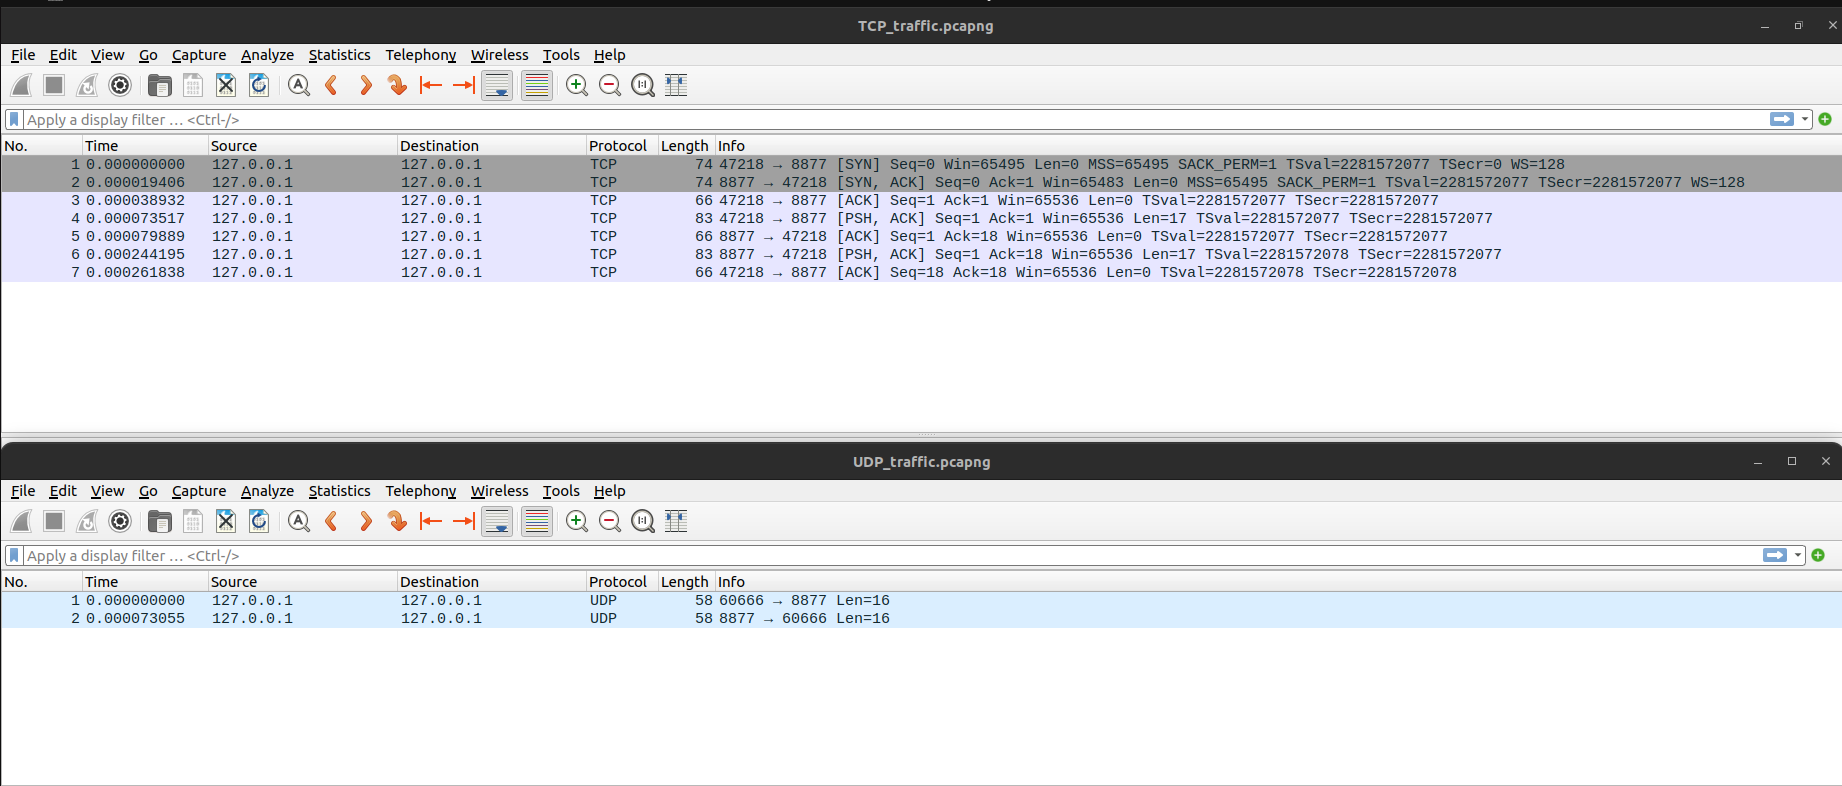
\includegraphics[width=\linewidth]{UDP-TCP.png}
  \caption{Comparaci�n entre el tr�fico UDP y TCP.}
  \label{fig:boat1}
\end{figure}

Para evitar posibles confusiones, modificamos los archivos cliente para que env�en un mismo mensaje (estructura de dos enteros en la que cada uno de ellos toma el valor 0) y observamos que para un tama�o de mensaje de 8 bytes, UDP emplea 100 bytes en 2 paquetes mientras que TCP emplea 494 bytes en 7 paquetes.

\begin{figure}[!h]
  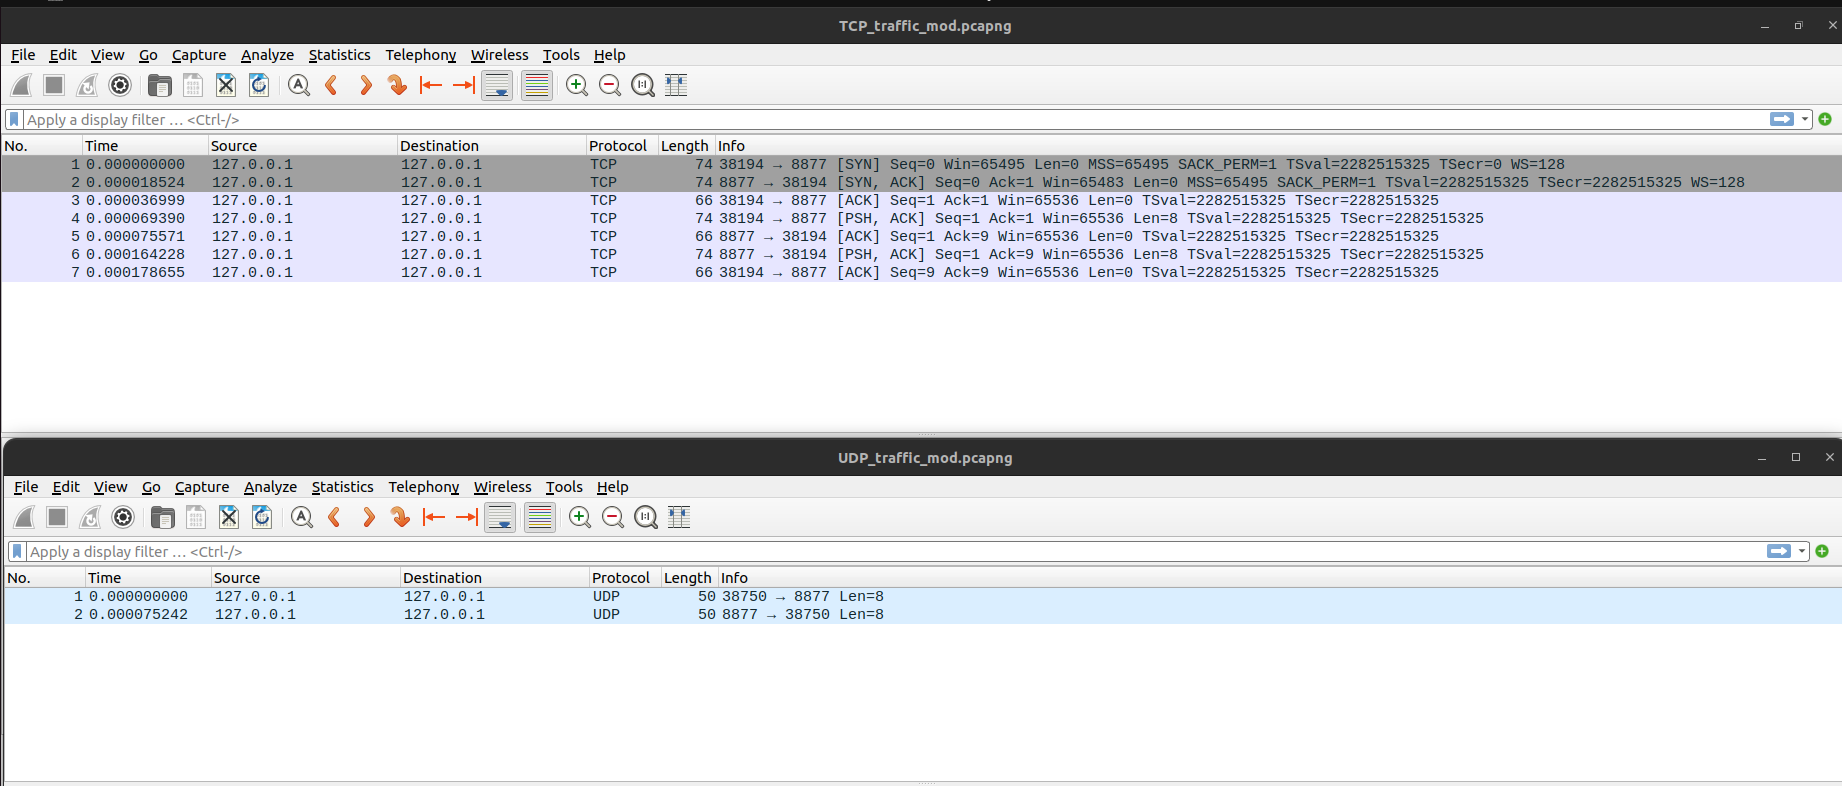
\includegraphics[width=\linewidth]{UDP-TCP-mod.png}
  \caption{Comparaci�n entre el tr�fico UDP y TCP con un mismo mensaje.}
  \label{fig:boat1}
\end{figure}

\newpage
\section{Generaci�n de una estructura compleja, env�o, captaci�n y muestra por pantalla}

Como ejercicio, se genera, de manera semialeatoria, una estructura que consta de cuatro entradas: un sello de tiempo, un entero, un caracter A-Z y un decimal. Tanto cliente como servidor mostrar�n por pantalla los valores recibidos. En este ejercicio para TCP observamos que la cantidad de mensajes que se pueden enviar depende del tama�o del buffer especificado, es decir, no generamos el buffer a medida que vamos careciendo de �l. Es por ello que, para UDP, s� que implementamos esta funcionalidad. 

\newpage
\section{Programaci�n de la tarjeta ESP-32}

Finalmente y partiendo de los proyectos ya desarrollados, hacemos que tanto cliente como servidor se implementen en la tarjeta ESP-32 proporcionada. En este caso nos decantamos por el protocolo UDP por el menor tr�fico de bytes. Desde menuconfig se conecta el servidor a la red deseada y se anota la IP que se le ha proporcionado al montar el proyecto; con esta IP y los datos anteriores, permitimos (tambi�n desde menuconfig) que el cliente se conecte con el servidor. Una vez establecida la conexi�n, el resto del trabajo consiste en copiar la estructura y adaptar el c�digo anterior.

\begin{figure}[!h]
  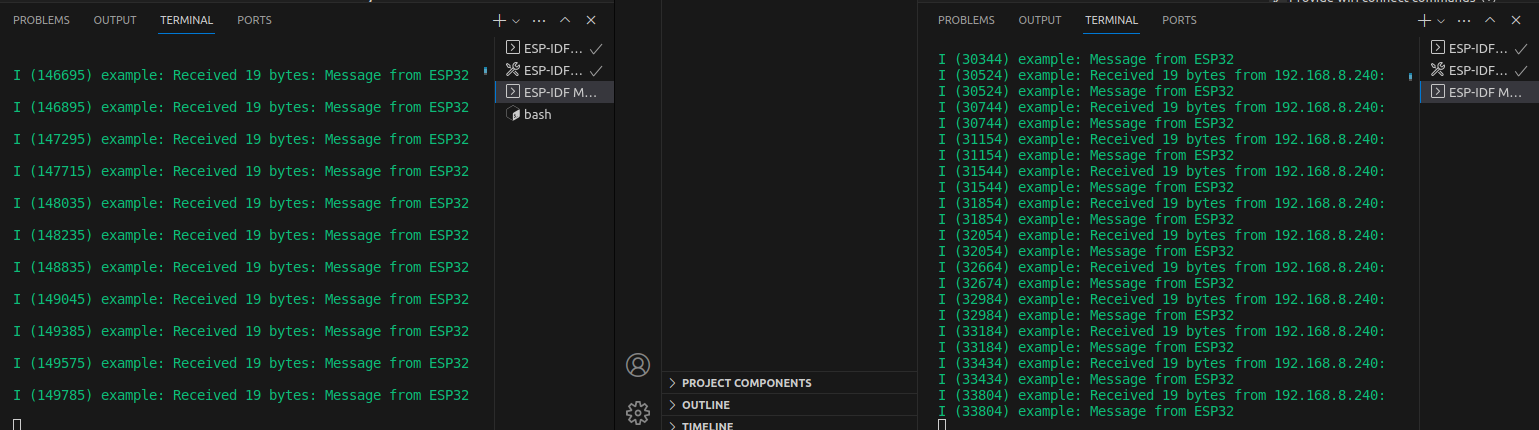
\includegraphics[width=\linewidth]{ConEst.png}
  \caption{Conexi�n establecida en ESP-32.}
  \label{fig:boat1}
\end{figure}








\end{document}
